\ExamPart{Câu trắc nghiệm nhiều phương án lựa chọn}{3}{Mỗi câu hỏi thí sinh chỉ chọn một phương án.}

\NQuestion Trong các hàm số sau, hàm số nào là hàm số bậc hai có trục đối xứng là đường thẳng $x=2$?

\ChoicesTwoLines
{$y=x^2-4x+1$.}
{$y=x^2+4x+1$.}
{$y=-x^2+2x+3$.}
{$y=2x^2+4x-5$.}

\NQuestion Cho phương trình $x^2-(m+1)x+m=0$. Giá trị nào của $m$ để phương trình có nghiệm kép?

\ChoicesOneLine{$m=1$.}{$m=-1$.}{$m=0$.}{$m=2$.}

\NQuestion Trong mặt phẳng tọa độ $Oxy$, cho điểm $A(2;-1)$ và vectơ $\vec u=(3;4)$. Tọa độ điểm $B$ thỏa mãn $\overrightarrow{AB}=\vec u$ là

\ChoicesOneLine{$B(5;3)$.}{$B(-1;-5)$.}{$B(1;3)$.}{$B(3;4)$.}

\NQuestion Trong mặt phẳng tọa độ $Oxy$, cho đường thẳng $\Delta:2x+3y-6=0$. Một vectơ pháp tuyến của $\Delta$ là

\ChoicesOneLine{$(2;3)$.}{$(3;-2)$.}{$(-3;2)$.}{$(1;1)$.}

\NQuestion Cho đường tròn $(C):x^2+y^2-4x+2y-4=0$. Bán kính của đường tròn bằng

\ChoicesOneLine{$3$.}{$5$.}{$\sqrt{5}$.}{$2\sqrt{6}$.}

\NQuestion Cho elip $(E):\dfrac{x^2}{36}+\dfrac{y^2}{20}=1$. Độ dài trục nhỏ của elip bằng

\ChoicesOneLine{$2\sqrt{5}$.}{$4\sqrt{5}$.}{$6$.}{$12$.}

\NQuestion Cho bất phương trình $x^2-6x+5>0$. Tập nghiệm của bất phương trình là

\ChoicesTwoLines
{$(-\infty;1)\cup(5;+\infty)$.}
{$[1;5]$.}
{$(1;5)$.}
{$(-\infty;1]\cup[5;+\infty)$.}

\NQuestion Cho hàm số bậc hai $y=f\left(x\right)$ có đồ thị như hình dưới đây. Mệnh đề nào sau đây đúng?

\begin{center}
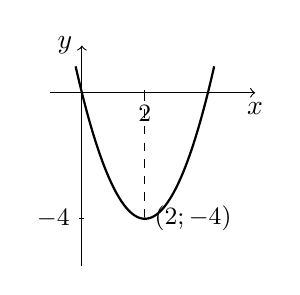
\begin{tikzpicture}[scale=0.4]
    \draw[->] (-1,0) -- (5.5,0) node[below] {$x$};
    \draw[->] (0,-5.5) -- (0,1.5) node[left] {$y$};

    \draw (2,0.08) -- (2,-0.08) node[below] {\small $2$};
    \draw (0,-4) ++(0.08,0) -- ++(-0.16,0) node[left] {\small $-4$};

    \draw[dashed] (2,0) -- (2,-4);
    \draw[thick, domain=-0.2:4.2, samples=200] plot (\x,{(\x-2)^2-4});

    \fill (2,-4) circle (1.3pt);
    \node[right] at (2,-4) {\small $(2;-4)$};
\end{tikzpicture}

\end{center}

\ChoicesTwoLines
{$f\left(x\right)$ đạt giá trị nhỏ nhất bằng $-4$ tại $x=2$.}
{$f\left(x\right)$ đạt giá trị lớn nhất bằng $-4$ tại $x=2$.}
{$f\left(x\right)$ đạt giá trị nhỏ nhất bằng $2$ tại $x=-4$.}
{$f\left(x\right)$ có hai cực trị.}

\NQuestion Một lớp có 6 học sinh giỏi Toán, 5 học sinh giỏi Văn và 4 học sinh giỏi Anh. Hỏi có bao nhiêu cách chọn ngẫu nhiên 1 học sinh từ nhóm trên để nhận thưởng?

\ChoicesOneLine{$15$.}{$120$.}{$30$.}{$24$.}

\NQuestion Trong mặt phẳng tọa độ $Oxy$, cho tam giác $ABC$ với $A(0;0)$, $B(4;0)$, $C(0;3)$. Diện tích tam giác $ABC$ bằng

\ChoicesOneLine{$6$.}{$12$.}{$7$.}{$\dfrac{7}{2}$.}
